\section{The SolarWinds operation}
\label{sec:operation}

\begin{figure}[t]
\centering
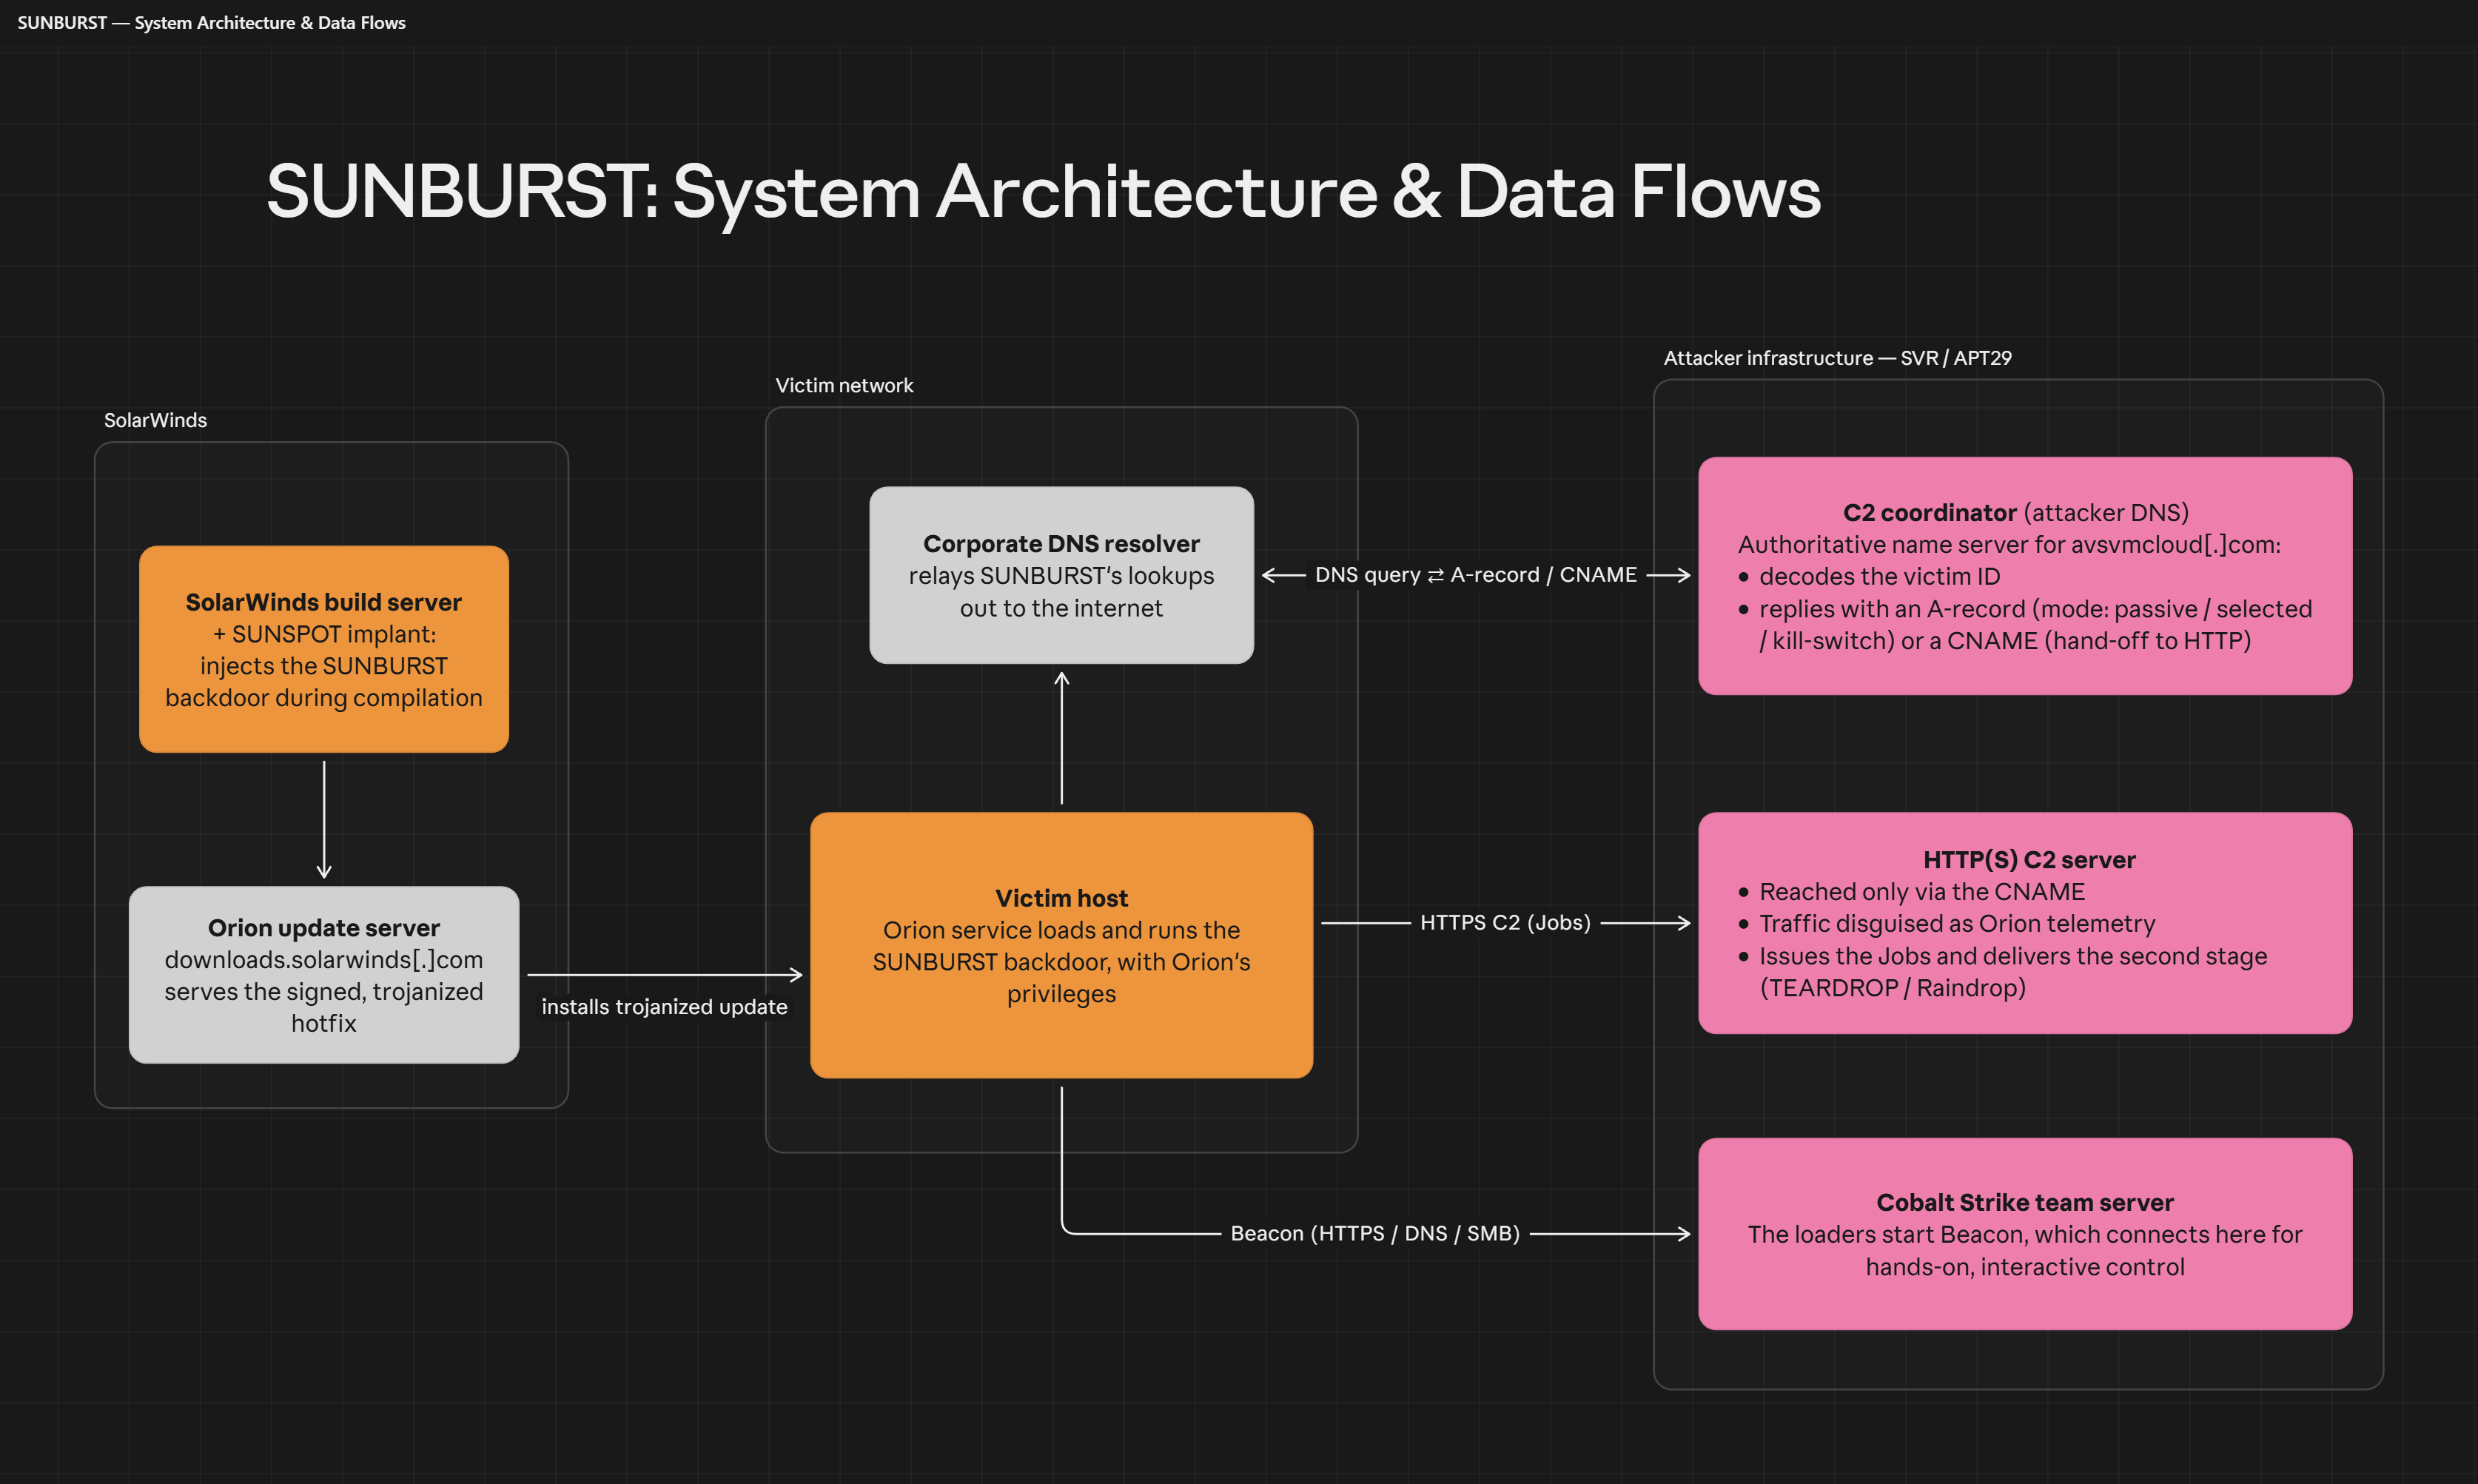
\includegraphics[width=0.92\textwidth,keepaspectratio]{architecture.png}
\caption{Attack architecture for the SolarWinds compromise, as documented in the Task~2 analysis. The build compromise precedes distribution; the lab in Section~\ref{sec:recreation} models the right-hand side of this path.}
\label{fig:architecture}
\end{figure}

Figure~\ref{fig:architecture} places the build compromise at the start of the chain: the actor works inside the supplier's environment, and every later stage inherits the supplier's legitimacy. The subsections below follow that path.

\subsection{Build compromise}

SolarWinds stated that it could not determine how the attackers first entered its network~\cite{solarwinds-sec}. CrowdStrike analysed an implant called SUNSPOT that ran on the Orion build server as \texttt{taskhostsvc.exe}, kept alive by a scheduled task. It waited for \texttt{MsBuild.exe}, read the build command line from process memory, and compared the MD5 of both the original source file and the backdoored copy against hardcoded values before replacing \texttt{InventoryManager.cs}. The original was kept as a \texttt{.bk} file and restored when the build exited, so the source repository looked untouched, and the edits were wrapped in \texttt{\#pragma warning disable}~\cite{crowdstrike-sunspot}.

The result was an Orion component containing SUNBURST. SolarWinds signed it through its normal release process and published it as a routine update~\cite{mandiant-campaign,mandiant-sunburst-details}.

\subsection{Dormancy and check-in}

SUNBURST did not act immediately. It required an Active Directory domain, stopped if the domain resembled a SolarWinds test environment, compared running processes against a list of analysis tools, and waited until the plugin file was 12 to 14 days old~\cite{mandiant-sunburst-details}. It then built a subdomain under \texttt{avsvmcloud[.]com} with a domain generation algorithm, encoding a user identifier and the victim's domain, and resolved it with the system DNS client~\cite{mandiant-sunburst-details}.

The coordinator answered with an A record, and the address range set the next state. Truncate (3) disabled the implant. New (4) kept it passive and checking in. Append (5) made it active. A CNAME response supplied the host for HTTPS command and control, which the malware required because it could not use a raw address~\cite{mandiant-sunburst-details}.

\subsection{Command and control and follow-on}

Active traffic imitated the Orion Improvement Program (OIP): JSON documents shaped like product telemetry, with fields such as \texttt{userId}, \texttt{sessionID}, and a \texttt{steps} array, and commands hidden in the response body. Payloads up to 10,000 bytes were wrapped as JSON; larger messages were sent unmodified. The tasking covered process execution, file transfer, registry access, and reboot~\cite{mandiant-sunburst-details}. On selected victims, operators delivered second-stage loaders. TEARDROP ran in memory, opened a file named \texttt{gracious\_truth.jpg}, and in at least one case used an Image File Execution Options value on \texttt{dllhost.exe} to start Cobalt Strike Beacon~\cite{microsoft-teardrop}. Raindrop was a second loader that served the same purpose~\cite{microsoft-teardrop}. Operators then used AdFind for directory enumeration and stole credentials including through DCSync~\cite{mandiant-campaign}. To reach Microsoft 365 mail, they compromised a SAML signing certificate and created valid tokens for accounts they did not control~\cite{cisa-aa20-352a}.

Exposure and compromise were different figures. Up to about 18,000 customers downloaded the affected builds, SolarWinds estimated that fewer than 100 were compromised, and nine U.S. federal agencies were among them~\cite{gao}.
